
\documentclass[11pt]{article}
\input{"../../preamble"}

% begin document
\begin{document}

% problem set 1
\section*{Problem Set 2}


\subsection*{Problem 1}
Let $\mathbf{u},\mathbf{v}$ be two vectors in $\mathbb{R}^{3}$. Compute $\mathbf{u}\times\mathbf{v}$, $\mathbf{u}\cdot\mathbf{v}$ for the following choices of $\mathbf{u}$ and $\mathbf{v}$, and state whether or not $\mathbf{u}$ and $\mathbf{v}$ are either orthogonal or colinear.

\begin{note}
  $u,v$ are orthogonal if $u\cdot v = 0$ and are colinear if $u\cdot v = \|u\| \|v\|$
\end{note}

\begin{enumerate}
  \item $\mathbf{u}=(6,0,−2)$, $\mathbf{v} = (0,8,0)$
  \begin{solution}
    \begin{align*}
      &u \cdot v = 6\times0 + 0\times8 + -2\times0 = 0 \\
      &u \times v = (0\times0-2\times8, 2\times0-6\times0, 6\times8-0\times0) = (-16, 0, 48)
    \end{align*}
  \end{solution}
  It is orthogonal and, therefore, not colinear

  \item $\mathbf{u}=(1,1,−1)$, $\mathbf{v} = (2,4,6)$
  \begin{solution}
    \begin{align*}
      &u \cdot v = 1*2 + 1*4 + -1*6 = 0\\
      &u \times v = (1*6-4*-1, -1*2-1*6, 1*4-2*1) = (10, -8, 2)
    \end{align*}
    It is orthogonal, and therefore, not colinear
  \end{solution}
\end{enumerate}


\subsection*{Problem 2}
Let $\vec{a}$, $\vec{b}$, $\vec{c}$, $\vec{d}$ $\in \mathbb{R}^{3}$ be vectors. Determine which of the following expressions are meaningless:
\begin{enumerate}
  \item $(\vec{a}\cdot \vec{b})\cdot \vec{c}$ \\
  Dot product is a number and can't dot product a vector
  \item $|\vec{a}|(\vec{b} \cdot \vec{c})$
  \item $\vec{a} \cdot(\vec{b}+ \vec{c})$
  \item $(\vec{a} \cdot \vec{b})\vec{c}$
  \item $\vec{a}\cdot \vec{b} + \vec{c}$
  cant add a scalar with a vector
  \item $\vec{a}\cdot (\vec{b}\times \vec{c})$
  \item $(\vec{a}\cdot \vec{b})\cdot (\vec{c}\cdot \vec{d})$ \\
  you cant dot product 2 numbers produced by dot product.
  \item $(\vec{a}\times \vec{b})\cdot (\vec{c}\times \vec{d})$
\end{enumerate}



\subsection*{Problem 3}
If $S$ is not closed, then there exists $x \in \overline{S}$ but $x \notin S$

\begin{proof}
  $ $\\
  If $S$ is not closed, then $S^c$ is not open. For a set $S^c$ to be open, every element in the set must be an interior of $S^c$. When $S^c$ is not open, then there exists an element in set $S^c$ such that $B_r(x) \not\subseteq S^c$, or that $B_r(x)\subseteq S$. Since closure of $S$, $\overline S = S\cup \partial S$, then $B_r(x)\in \overline S$. Also since $s\in S^c$, then $s\not\in S$. Therefore there exists $x\in \overline S \land x\not\in S$
\end{proof}


\subsection*{Problem 4}
Prove that for any $x,y \in \mathbb{R}^{n}$, $\vert x - y \vert \geq \big\vert \vert x \vert - \vert y \vert \big\vert$. This is commonly called, \textbf{the reverse triangle inequality}. It is extremely useful when you want to prove inequalities like $\vert (x-a)^{-1} \vert \leq M$ for $x$ in some fixed closed set.

\begin{proof}
  $ $\\
  \begin{align*}
    \| x-y \| &= \sqrt{(x-y)\cdot (x-y)} \tag{Norm definition} \\
    &= \sqrt{x\cdot x -2x\cdot y + y\cdot y}     \tag{properties of vector space}\\
    &\lgeq \sqrt{\| x \|^2 - 2\|x\| \|y\| + \|y\|^2} \tag{Couchy Schwarz Inequality} \\
    &= \sqrt{(\|x\|-\|y\|)^2} \\
    &= \big\vert \|x \| - \|y \| \big\vert
  \end{align*}
\end{proof}


\subsection*{Problem 5}

If $U$ and $V$ are open (resp. closed) then $U\cup V$ is open (resp. $U\cap V$ is closed). If $\left\{U_{i}\right\}_{i\in I}$ is a countable collection of open sets, must $\bigcap_{i\in I}U_i$ be open? Provide a proof or counterexample. Similarly, if $\left\{A_{i}\right\}_{i\in I}$ is an infinite collection of closed sets, must $\bigcap_{i\in I}A_i$ be closed?

$ $\\
\textbf{Prove} If $U$ and $V$ are open, then $U\cup V$ is open.
\begin{proof}
  $ $\\
  Let $x\in U\cup V$, then $x\in U \lor x\in V$. If $x\in U$, then $\exists r > 0, B_r(x)\in U$ because $U$ is open. If $x\in V$, then $\exists r > 0, B_r(x)\in V$ because $V$ is open. Therefore $\forall x\in U\cup V, \exists r>0, B_r(x)\in U\cup V$, which means that $U\cup V$ is open. If a set is open then its complement is closed. Therefore $(U\cup V)^c = U^c \cap V^c$. Since $U\cup V$ is open. $(U\cup V)^c$ is closed. Also $U^c, V^c$ are closed. Then intersection of them is closed.
\end{proof}
$ $\\
\textbf{Prove} If $\left\{U_{i}\right\}_{i\in I}$ is a countable collection of open sets. There are cases when the union is closed.
\begin{proof}
  $ $\\
  However for countable collection of open set $\left\{U_{i}\right\}_{i\in I}$, although maybe intuitive to think that it is open, have exceptions. For example when $U_n = (-\frac{1}{n}, \frac{1}{n})$. It is apparent that for any $n$ open interval $U_n$ is an open set. To prove this let $x\in \R$ such that $-\frac{1}{n}<c<\frac{1}{n}$ for any $n$ and $\epsilon>0$, take $\epsilon = \frac{1}{2} \text{min}( \frac{1}{n} - x, x - \frac{1}{n} ) $. Let $B_{\epsilon}(c) = \{ y\in \R, \| y-c\| < \epsilon\} =(c-\epsilon, c+\epsilon)$ be an open ball of $c$. We have $c+\epsilon < \frac{1}{n}$ and $c-\epsilon > -\frac{1}{n}$. Therefore $B_{\epsilon}(c)\subseteq (-\frac{1}{n}, \frac{1}{n})$. We can conclude any interval $U_n$ is an open set. $\{U_i\}_{i\in I} = \{ 0 \}$ as $n \to \infty$. It's easy to prove that a set with one element is closed
\end{proof}
$ $\\
\textbf{Prove} If $\left\{A_{i}\right\}_{i\in I}$ is an infinite collection of closed sets, $\bigcap_{i\in I}A_i$ must be closed.

\begin{proof}
  $ $\\
  If $\left\{A_{i}\right\}_{i\in I}$ is an infinite collection of closed sets, then $\{ A_i^c\}_{i\in \I}$ must be a collection of open sets. Then $\forall x\in A_i^c$ such that $\exists r > 0, B_r(x) \in A_r^c$ for any $i\in\I$. Therefore $B_r(x)\subseteq \bigcup_{i\in\I}(A_i^c)$ for any $x\in \bigcup_{i\in\I}(A_i^c)$, which means $\bigcup_{i\in\I}(A_i^c)$ is open. Therefore $\bigg(\bigcup_{i\in\I}(A_i^c)\bigg)^c = \bigcap_{i\in \I}A_i$ is closed.

\end{proof}



\end{solution}



\subsection*{Problem 6}

Prove that the following sets are open,

\begin{rem}
  Proving that a set is open requires proving that every point within the set is an interior point, or that there exists open ball centered at point and that the ball is contained in the set.
\end{rem}

\begin{enumerate}
  \item $\R^n$
  \begin{proof}
    $ $\\
    Take an arbitrary vector $v\in \R^n$. Let $r>0$, claim that $B_r(v) \subseteq \R^n$. Proof by contradiction. Let $w\not\in \R^n \land w\in B_r(v)$. Since $ w\in B_r(v)$, $\|w-v\| < r$. Here contradiction arises because metric only applies to vectors in the same dimension. Therefore $\R^n$ is open. Let $y' \in B_r(x)$
  \end{proof}

  \item $B_r(x)$
  \begin{proof}
    $ $\\
    Let $x\in \R^n$ and $r>0$ be arbitrary. And consider $B_r(x)$. Need to show that $\forall y\in B_r(x): \exists r' > 0: B_{r'}(y)\in B_r(x)$ Let arbitrary $y\in B_r(x)$, and by definition, $d = \| y - x \| < r$. Let $r' = \frac{r-d}{2}$. We claim that any arbitrary element in $p\in B_{r'}(y)$ will also be contained in $B_r(x)$. To prove this, we show
    \begin{align*}
      \|p-x\| &= \| p + y - y -x \| \\
      &\leq \| p-y\| + \| y-x\| \tag{triangular inequality}\\
      &\leq r' + d \tag{$d = \| y-x\|$ and $\|p-y\| \leq r'$} \\
      &= \frac{r-d}{2} + d \\
      &= \frac{r+d}{2} \\
      &\leq r \tag{$d<r$}
    \end{align*}
    Therefore we proved any open ball is open.
  \end{proof}

  \item $\{(x,y)\in \R^2: x > 0\}$
  \begin{proof}
    $ $\\
    Let $S=\{ (x,y)\in \R^2: x > 0\}$. Take arbitrary $p = (x,y)\in S$, let $r=\frac{x}{2}$. We claim that $B = B_r(p) \in S$. To prove this, we take an arbitrary point in $q = (v, w)\in B$ and prove that $(v, w)\in S$. If $v > x$, then $v>0$ because $x >0$ by definition. If $v < x$, because $q\in B$,
    \begin{align*}
      | v-x | &< r \\
      x - v &< \frac{x}{2} \tag{$r = \frac{x}{2}$}\\
      v &> \frac{x}{2} > 0 \tag{$x>0$}
    \end{align*}
    Then $q\in S$. Therefore $q\in B \Rightarrow q\in S$. Any arbitrary element in $S$ has a ball centered at itself and the ball is contained in $S$. We proved $\{ (x,y)\in \R^2: x > 0\}$ is open.
  \end{proof}

  \item $\{(x,y)\in \R^2: x > 1 \land y>0\}$
  \begin{proof}
    $ $ \\
    Since $\{(x,y)\in \R^2: x > 1 \land y>0\} = \{ (x,y)\in \R^2 x > 1\} \cap \{ (x,y)\in \R^2 y > 0\}$. We prove the composing subsets are open as seen in the previous question. Since intersection of open sets are also open, we proved this question.
  \end{proof}

  \item $S = \{ (x,y): x\not\in \mathbb{Z}\}$
  \begin{proof}
    $ $\\
    Let $p = (a,b)\in S$, thus $a\not\in \mathbb{Z}$. $\exists n \in \mathbb{Z}, n < a < n+1$. Let $r=\frac{1}{2} min(n+1-a, a - n)$. We claim that $B_r(p) \subseteq S$. Let arbitrary $q = (v,w) \in B_r(p)$. Then $v\in (a-r, a+r)$. Since $n < a-r \land n < a+r$ because of $r$ assigned. Then $n< v < n+1$, or $n\not\in \mathbb{Z}$. Proved.
  \end{proof}
\end{enumerate}


\subsection*{Problem 7}
Determine and prove whether the following sets are open, closed, or neither open nor closed

\begin{enumerate}
  \item $S = \{ (x,y): x\in \mathbb{Z}\}$
  \begin{proof}
    $ $ \\
    Set $S$ is closed if the complement $S^c = \{ (x,y): x\not\in \mathbb{Z}\}$ is open, which is proved in the last problem.
  \end{proof}

  \item  $S = \{ (x,y): x^2 + y^2 = 1\}$
  \begin{proof}
    $ $\\
    \begin{center}
      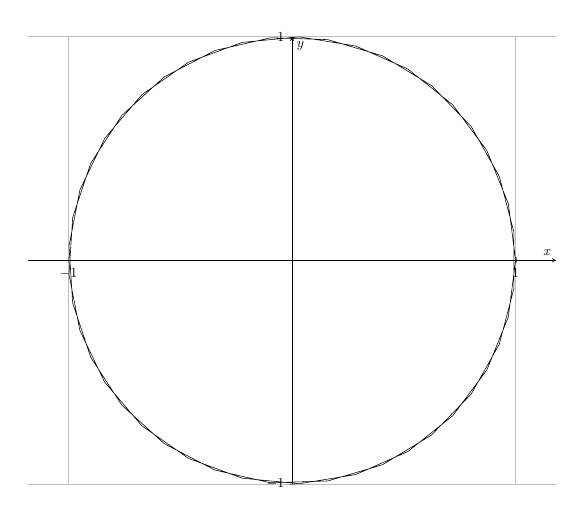
\begin{tikzpicture}[scale=0.5]
        \begin{axis}[
          width=15cm,               %% here, adjust as suitable
          %axis y line=center,
          %axis x line=middle,
          axis lines = middle,  %% instead of above two lines this one is enough
          scaled ticks=false,
          axis equal,
          grid=major,
          xmax=1,xmin=-1,
          ymin=-1,ymax=1,
          xlabel=$x$,ylabel=$y$,
          xtick={-1,...,1},
          ytick={-1,...,1},
          ]
          \addplot [domain=0*pi:4*pi,samples=50]({cos(deg(x))},{sin(deg(x))});
        \end{axis}
      \end{tikzpicture}
    \end{center}
    Claim the set is closed. We prove that the complement $S^c = \{ (x,y): x^2 + y^2 \neq 1\}$ is open. The set can also be written this way $S^c = \{ p\in \R^2: \|p\| \neq 1\} = \{ p\in \R^2: \|p\| < 1\}\cup \{ p\in \R^2: \|p\| > 1\}$.
    \begin{case}
      $S_1  = \{ p\in \R^2: \|p\| < 1\}$ \\
      Because an open ball is an open set and $S_1$ is basically an open ball centered at the origin with radius of 1. Therefore $S_1$ is open.
    \end{case}
    \begin{case}
      $S_2  = \{ p\in \R^2: \|p\| > 1\}$ \\
      Let $p\in S_2$. We define $d = \|p \|$. Let $r=\frac{d-1}{2}$. We claim that $B_r(p)\subseteq S_2$. To prove this we let arbitrary $q\in B_r(p)$, then we have $\|p-q\| < r = \frac{d-1}{2}$. Now we prove that $\|q\| > 1$. There are two cases. When $\|q\| > \|p\|$, then $\|q\| > 1$ because $\|p\| > 1$. When $\|q\| < \|p\|$,
      \begin{align*}
        \| q \| + \| p-q\| &\geq \|p\| \tag{Triangular inequality}\\
        \| q\| + \frac{d-1}{2} &\geq d\tag{$\|p\| = d \land \|p-q\| \leq r = \frac{d-1}{2}$} \\
        \|q\| &\geq \frac{d+1}{2} \\
        \|q\| &> 1 \tag{$d>1$}
      \end{align*}
      Therefore $q\in S_2$. Then $S_2$ is open. \\
    \end{case}
    The union of two open sets are open as proved previously. Then $S$ is open.
  \end{proof}

  \item $S = \{ (x,y): x^2 + y^2 \leq 1\}$
  \begin{proof}
    $ $ \\
    We claim that $S$ is closed, which is same as proving $S^c = \{ (x,y)\in \R^2: x^2 + y^2 > 1\}$ is open, which we proved in the previous question.
  \end{proof}

  \item $S = \{ (x,y): x^2 + y^2 \leq 1 \land (x,y) \neq (0,0)\}$
  \begin{proof}
    $ $\\
    $S$ is neither open nor closed \\
    CASE 1:
      $S$ is not open \\
      $S$ not open implies that $\exists x\in S: \forall r>0, B_r(x)\not\subseteq S$. Let $p = (x,y)\in S$ such that $x^2 + y^2 = 1$, which means that $p\in S$. for arbitrary $r>0$, $B_r(p)\cap S \neq \emptyset$ because $p\in B_r(p) \land p\in S$. We also claim $B_r(p)\cap S^c \neq \emptyset$ for any $r>0$. Let arbitrary $q = (v,w)\in B_r(p)$ such that $\|q\| > \|p\|$. Then $v^2 + w^2 > 1$, which means $q\in S^c$. Therefore $B_r(p)\cap S^c \neq \emptyset$. Then $p$ is a boundary point, and not an interior point. Not every element of $S$ is an interior point, therefore $S$ is not open. \hilight{is this right?} \\
    CASE 2:
      $S$ is not closed \\
      Proof by contradiction. If $S$ is closed, then $\partial S \in S$, which means that every boundary point of $S$ is in $S$. Consider $p = (0,0)$, which we claim to be a boundary point of $S$. Let $B = B_r(p)$ be a ball centered at $p$ with any $r>0$. We can show that $B\cap S^c \neq \emptyset$ because $\{(0,0)\} \subseteq S^c \land \{(0,0)\}\subseteq B$. We can also show that $B\cap S \neq \emptyset$. Let $q = (v,w)\in B_r(p)$ with an arbitrary $r>0$ such that $1> \|q-p\| > 0$. Then $1 > \|q\| = v^2 + w^2 > 0$. Then $\exists q \in S$. We proved that $B\cap S \neq \emptyset$. Therefore $p$ is a boundary point of $S$. However $p\in S^c$, this contradict with assumption that every boundary point of $S$ is in $S$. We proved that $S$ is not closed.
  \end{proof}

  \item $S = \{ (x,y): x>0 \land y=sin(\frac{1}{x})\}$
  \begin{proof}
    $ $\\
    \begin{center}
      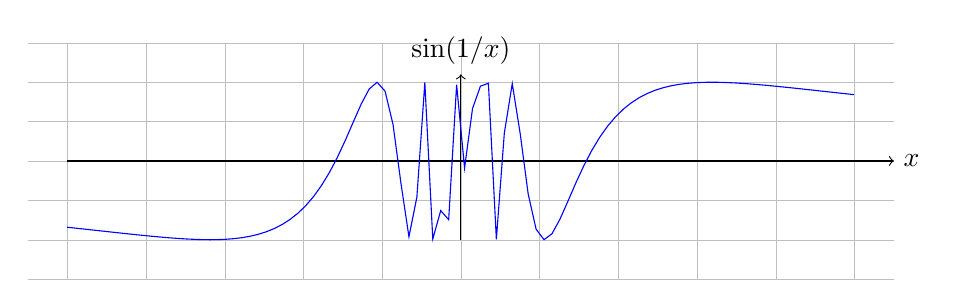
\begin{tikzpicture}[x=5cm]
          \draw[xstep=.2,ystep=.5,lightgray,ultra thin] (-1.1,-1.5) grid (1.1,1.5);
          \draw[->] (-1,0) -- (1.1,0) node[right] {$x$};
          \draw[->] (0,-1) -- (0,1.1) node[above] {$\sin (1/x)$};
        \draw[blue,domain=-1:1,samples=100] plot (\x, {sin((1/\x)r)});
      \end{tikzpicture}
    \end{center}

    \hilight{dunno how to prove this..}
  \end{proof}


  \item $S = \{ (x,y): 0<x<1 \land 0<y<1 \land x,y\in \mathbb{Q})\}$

  \begin{proof}
    $ $\\
    $S$ is neither open nor closed. $S$ is not closed $\exists x\not\in S, x\in \partial S$. An example of this would be $p=(1,1)$. $B=B_r(p)$ for any arbitrary $r>0$. $B\cap S^c \neq \emptyset$ because $p$ is contained in both set. $B\cap S\neq \emptyset$ because $\exists q=(v,w)$ such that $v<1, w<1$ and $\|q-p\| < r \land v,w\in \mathbb{Q}$. These two condition does not conflict with each other. \hilight{can i say this though..} Therefore not all boundary point of $S$ is contained in $S$, then $S$ is not closed. To prove $S$ is not open, we take arbitrary $t\in S$. We prove that $B_r(t) \not\subseteq S$ for any $r>0$. Proof by contradiction: we assume $B_r(t) \subseteq S$. Let $z\in B_r(t)$ such that $z\not\in \mathbb{Q}$. This is possible because real numbers are dense. And a ball of any radius would contain both rational and irrational number. This is a contradiction since $z\in S$, meaning that $z\in \mathbb{Q}$ by definition. Therefore $B_r(t) \not\subseteq S$ for some $t\in S$
  \end{proof}

  \item $S = \{ (x,y): y > x^2)\}$
  \begin{proof}
    $ $\\
    \hilight{how to prove this formally?}
    $S$ is open. Let $P=\{ (x,y): y=x^2\}$ and we set claim $T(x)$ to be $inf\{ \|x - t\| : t\in P\}$. Let arbitrary $s\in S$ and make $r= T(x)$. Let $B_r(s)$ be an open ball. We claim that $B_r(s)\subseteq S$ For arbitrary $v\in B_r(s)$. .... uhh
  \end{proof}
\end{enumerate}


\subsection*{Problem 8}
Construct an open set of arbitrarily small \"size\" which contains the rational numbers $\mathbb{Q}$, but which is a proper subset of $\mathbb{R}$. In this context we define the size of $(a,b)$ for $a < b$ to be $b-a$. We define the size of a union of open intervals to be the sum of their sizes.

\begin{solution}
  $ $\\
  Let us understand what we should do. Start with $S=\{ x\}$. Let $\epsilon > 0, u = (x-\frac{\epsilon}{2}, x+\frac{\epsilon}{2})$. Let $S=\{ x_1, x_2\}$, $(x_1 - \frac{\epsilon}{4}, x_1 + \frac{\epsilon}{4}) \cup (x_2 - \frac{\epsilon}{4}, x_2 + \frac{\epsilon}{4}) \leq \frac{\epsilon}{2} + \frac{\epsilon}{2} = \epsilon$. Let $S=\{ x_1, x_2, \dots, x_n\}$. $\sum_{n=0}^{\infty}{\frac{1}{2^n}}$ converges to 1. So find intervals length $\frac{\epsilon}{2^{n+1}}$. $\bigcup_{n=0}(x_n-\frac{\epsilon}{2^{n+1}}, x_n + \frac{\epsilon}{2^{n+1}}) \leq \epsilon \sum_{n=0}^{\infty}(\frac{1}{2^n}) = \epsilon$. $Q$ is countable. Let's enumerate the rationals $Q = \{ r_1, r_2, \dots\}$

  \hilight{dont really understand this...}
\end{solution}






% end document
\end{document}
